% Created 2021-10-26 mar. 15:12
% Intended LaTeX compiler: pdflatex
\documentclass[10pt]{beamer}
\usepackage[utf8]{inputenc}
\usepackage[T1]{fontenc}
\usepackage{graphicx}
\usepackage{grffile}
\usepackage{longtable}
\usepackage{wrapfig}
\usepackage{rotating}
\usepackage[normalem]{ulem}
\usepackage{amsmath}
\usepackage{textcomp}
\usepackage{amssymb}
\usepackage{capt-of}
\usepackage{hyperref}
\usepackage{minted}
\setlength{\parskip}{5pt}
\newcommand{\footnoteframe}[1]{\footnote[frame]{#1}}
\addtobeamertemplate{footnote}{}{\vspace{2ex}}
\usepackage{tabularx}
\usetheme{Berkeley}
\author{Jay Morgan}
\date{11th October 2021}
\title{Programming Level-up}
\subtitle{Lecture 3 -- Modules \& Development Environments}
\hypersetup{
 pdfauthor={Jay Morgan},
 pdftitle={Programming Level-up},
 pdfkeywords={},
 pdfsubject={},
 pdfcreator={Emacs 27.1 (Org mode 9.4.6)}, 
 pdflang={English}}
\begin{document}

\maketitle
\begin{frame}{Outline}
\tableofcontents
\end{frame}


\section{Modules}
\label{sec:org1895584}

\subsection{Python Modules}
\label{sec:org57f0b5e}

\begin{frame}[label={sec:org7094c73}]{Importing in python}
\begin{center}
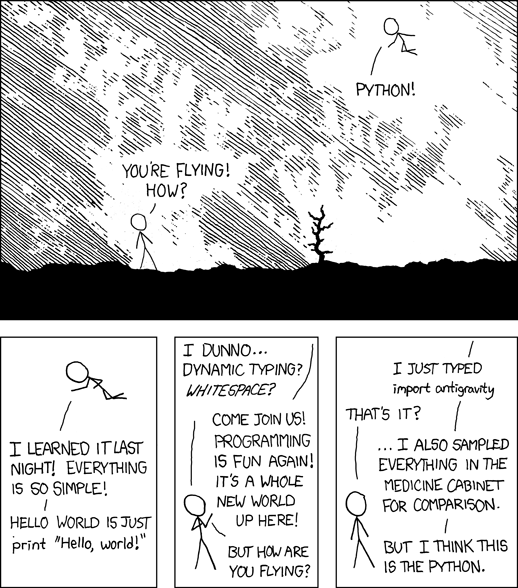
\includegraphics[width=0.6\textwidth]{images/python.png}
\end{center}
\url{https://xkcd.com/353/}
\end{frame}

\begin{frame}[label={sec:orgd8daac0},fragile]{The basic structure of importing}
 Modules or packages are other \emph{scripts or programs} that can be imported into other
scripts. This definition is very general, but we shall see how flexible importing in
Python can be.

The basic syntax of importing is:

\begin{minted}[frame=lines,linenos=true,firstnumber=last,fontsize=\footnotesize,xleftmargin=15pt,numbersep=8pt]{python}
import <package_name>

<package_name>.<function/class/variable/etc>
\end{minted}

If we import \texttt{<package\_name>} using this syntax, we always have to use the dot \texttt{.} syntax
to refer to something within this package.
\end{frame}

\begin{frame}[label={sec:org09bd422},fragile]{The basic structure of importing}
 Let's take a look at a very basic example.

\begin{minted}[frame=lines,linenos=true,firstnumber=last,fontsize=\footnotesize,xleftmargin=15pt,numbersep=8pt]{python}
import math

radius = 6.4  # cm
circum = 2 * math.pi * radius
\end{minted}

In this example, we are importing the built-in \texttt{math} package. This package contains a
bunch of useful functions and variables. We're not going to take a look at them
here, as we're focusing on importing, but you can see we're referring to a variable
called \texttt{pi} to calculate the circumference of a circle.
\end{frame}

\begin{frame}[label={sec:orgf1a8738},fragile]{Importing specific items}
 If we didn't always want to specify the package name when we only want to use
something specific from a package, we can directly import that something.

\begin{minted}[frame=lines,linenos=true,firstnumber=last,fontsize=\footnotesize,xleftmargin=15pt,numbersep=8pt]{python}
from <package_name> import <function/class/variable/etc>

<function/class/variable/etc>
\end{minted}

As you can see, we're using the \texttt{from ... import ...} syntax.

\begin{minted}[frame=lines,linenos=true,firstnumber=last,fontsize=\footnotesize,xleftmargin=15pt,numbersep=8pt]{python}
from math import pi

circumference = 2 * pi * radius
\end{minted}
\end{frame}

\begin{frame}[label={sec:orgba4271d},fragile]{Don't do this!}
 When using \texttt{from ... import ...}, there is a wildcard \texttt{*} that we \alert{could} use. You may
sometimes see this style of importing when looking at documentation online:

\begin{minted}[frame=lines,linenos=true,firstnumber=last,fontsize=\footnotesize,xleftmargin=15pt,numbersep=8pt]{python}
from <package_name> import *

<function/class/variable/etc>
\end{minted}

However, this can create many problems with reading your program code
\end{frame}

\begin{frame}[label={sec:org223aee5},fragile]{Don't do this!}
 Which module does \texttt{my\_function()} originate? Are there are common names between the
two? Which would be used?

\begin{minted}[frame=lines,linenos=true,firstnumber=last,fontsize=\footnotesize,xleftmargin=15pt,numbersep=8pt]{python}
from my_module import *
from my_second_module import *

my_function()
\end{minted}
\end{frame}

\begin{frame}[label={sec:org76af65d},fragile]{Alias}
 When importing, we can optionally create an alias to a symbol. Here we're creating an
alias to the existing \texttt{pi} in \texttt{math}.

\begin{minted}[frame=lines,linenos=true,firstnumber=last,fontsize=\footnotesize,xleftmargin=15pt,numbersep=8pt]{python}
from math import pi as decilious_pi

circumference = 2 * delicious_pi * radius
\end{minted}

There are some very common conventions of aliasing very highly used packages that we
will definitely revisit in another lecture!

\begin{minted}[frame=lines,linenos=true,firstnumber=last,fontsize=\footnotesize,xleftmargin=15pt,numbersep=8pt]{python}
import numpy as np
import pandas as pd
import matplotlib.pyplot as plt
\end{minted}
\end{frame}

\begin{frame}[label={sec:org5fe7f88},fragile]{Importing local libraries}
 let's consider a hypothetical local directory:

\begin{minted}[frame=lines,linenos=true,firstnumber=last,fontsize=\footnotesize,xleftmargin=15pt,numbersep=8pt]{bash}
main.py
src/
 |-- my_module.py
 |-- module_1/
	|-- cats.py
	|-- dogs.py
\end{minted}

If we wanted to import something from \texttt{my\_module.py} we would do:

\begin{minted}[frame=lines,linenos=true,firstnumber=last,fontsize=\footnotesize,xleftmargin=15pt,numbersep=8pt]{python}
from src.my_module import MyAwesomeClass

my_class = MyAwesomeclass()
\end{minted}
\end{frame}

\begin{frame}[label={sec:org7c53d67},fragile]{Importing local libraries}
 \begin{minted}[frame=lines,linenos=true,firstnumber=last,fontsize=\footnotesize,xleftmargin=15pt,numbersep=8pt]{bash}
main.py
src/
 |-- my_module.py
 |-- module_1/
	|-- cats.py
	|-- dogs.py
\end{minted}

Here is another example for increased nesting of directories:

\begin{minted}[frame=lines,linenos=true,firstnumber=last,fontsize=\footnotesize,xleftmargin=15pt,numbersep=8pt]{python}
from src.module_1 import cats
from src.module_1.dogs import Dog

cat = cats.Cat()
dog = Dog()
\end{minted}
\end{frame}


\begin{frame}[label={sec:orgb893a98},fragile]{Quick exercise -- imports}
 \begin{itemize}
\item Create a directory to store your scripts
\item In this directory, create a file called \texttt{main.py}.
\item Create a sub-directory called \texttt{src}. In \texttt{src} create another file called \texttt{library.py}.
\item In \texttt{library.py} create a class (that doesn't do anything right now) called \texttt{Database}.
\item In \texttt{main.py}, create an instance of \texttt{Database}.
\end{itemize}
\end{frame}

\begin{frame}[label={sec:org43fcbad},fragile]{Shortcuts with \texttt{\_\_init\_\_.py}}
 Let's say you often import \texttt{Cat} and \texttt{Dog}. We can use a file called \texttt{\_\_init\_\_.py} to help
us and make the imports shorter. This fill gets executed when its module is imported.

\begin{minted}[frame=lines,linenos=true,firstnumber=last,fontsize=\footnotesize,xleftmargin=15pt,numbersep=8pt]{bash}
main.py
src/
 |-- my_module.py
 |-- module_1/
	|-- __init__.py
	|-- cats.py
	|-- dogs.py
\end{minted}

In \texttt{\_\_init\_\_.py}:

\begin{minted}[frame=lines,linenos=true,firstnumber=last,fontsize=\footnotesize,xleftmargin=15pt,numbersep=8pt]{python}
from cats import Cat
from dogs import Dog
\end{minted}

In \texttt{main.py}:

\begin{minted}[frame=lines,linenos=true,firstnumber=last,fontsize=\footnotesize,xleftmargin=15pt,numbersep=8pt]{python}
from src.module_1 import Cat, Dog
\end{minted}
\end{frame}

\begin{frame}[label={sec:org834e2ab},fragile]{What is \texttt{\_\_main\_\_}?}
 Consider a file with the following:

\begin{minted}[frame=lines,linenos=true,firstnumber=last,fontsize=\footnotesize,xleftmargin=15pt,numbersep=8pt]{python}
x = 2
y = 1
z = x + y

class MyAwesomeClass:
    ...
\end{minted}

If we import this file in another script, \texttt{x, y,} and \texttt{z} will be computed. In this very
simple case this will have very little impact. But what if the computation of these
takes a very long time?
\end{frame}

\begin{frame}[label={sec:orgc6f7ca4},fragile]{What is \texttt{\_\_main\_\_}?}
 Here we are wrapping any global computations into a appropriate functions. This
prevents the global variables being computed as soon as the script is imported.

Now, if we wanted to compute x, y, and z if this script is run, we could use:

\begin{minted}[frame=lines,linenos=true,firstnumber=last,fontsize=\footnotesize,xleftmargin=15pt,numbersep=8pt]{python}
if __name__ == "__main__":
    # do something
\end{minted}

Anything within the scope of the \texttt{if} function will only be run if the current file is
the script that is being run directly (i.e. \texttt{python <the-file>.py}). If the script is
being imported, the statements within this if scope will not be run.
\end{frame}

\begin{frame}[label={sec:orgac9ef50},fragile]{What is \texttt{\_\_main\_\_}?}
 So if we wanted to run \texttt{compute()} if this file is being run directly, we would write:

\begin{minted}[frame=lines,linenos=true,firstnumber=last,fontsize=\footnotesize,xleftmargin=15pt,numbersep=8pt]{python}
def compute():
    x = 2
    y = 1
    z = x + y

class MyAwesomeClass:
    ...

if __name__ == "__main__":
    compute()
    # we can of course use MyAwesomeClass as well
    my_class = MyAwesomeClass()
    my_class.do_something()
\end{minted}
\end{frame}

\section{Working with Files and Directories}
\label{sec:org8e506bd}

\subsection{Paths}
\label{sec:org4182fdf}

\begin{frame}[label={sec:org84efd6a},fragile]{Current working directory}
 The folder in which you run Python will be the \emph{current working directory (CWD)}. We can
print this value with the \texttt{os.getcwd()} function, or change the directory with
\texttt{os.chdir(...)}. Its important to know what your CWD is as all relative paths (paths
that do not start with a '/') will be relative to your CWD.

\begin{minted}[frame=lines,linenos=true,firstnumber=last,fontsize=\footnotesize,xleftmargin=15pt,numbersep=8pt]{python}
import os

print(os.getcwd())
os.chdir("../")
print(os.getcwd())
os.chdir("week-3")
\end{minted}

\begin{verbatim}
Results: 
# => [...]/Programming Level-up/week-3
# => [...]/Programming Level-up
\end{verbatim}


I've replaced the full path printed by Python with \texttt{[...]} so you can see the
differences in the paths!
\end{frame}

\begin{frame}[label={sec:orge63d75c},fragile]{Listing directories}
 Continuing with our usage of the \texttt{os} package, we can use the \texttt{listdir} function to list
all files within a directory.

\begin{minted}[frame=lines,linenos=true,firstnumber=last,fontsize=\footnotesize,xleftmargin=15pt,numbersep=8pt]{python}
print(os.listdir())
print(os.listdir("images/"))
\end{minted}

\begin{verbatim}
Results: 
# => ['images', '__pycache__', 'lecture.pdf', 'lecture.tex', 'data', 'test_file_1.py', 'lecture.org', '_minted-lecture', 'test_file_2.py']
# => ['legend-2.png', 'fig-size.png', 'basic.png', 'subplots.png', 'python.png', 'pycharm01.png', 'installing-scikit-learn.png', 'pycharm02.png', 'PyCharm_Icon.png', 'axis.png', 'legend.png', 'complex-pycharm.jpg']
\end{verbatim}


This returns a list of files and directory relative to your current working
directory. Notice how from this list you cannot tell if something is a file or
directory (though the filename does provide some hint).
\end{frame}

\begin{frame}[label={sec:org7857488},fragile]{Testing for files or directories}
 In the previous example we saw that the items returned by \texttt{listdir} does not specify if
the item is a file or directory. However, \texttt{os} provides an \texttt{isfile} function in the \texttt{path}
submodule to test if the argument is a file, else it will be a directory.

\begin{minted}[frame=lines,linenos=true,firstnumber=last,fontsize=\footnotesize,xleftmargin=15pt,numbersep=8pt]{python}
for path in os.listdir():
    print(f"{path} => is file: {os.path.isfile(path)}")
\end{minted}

\begin{verbatim}
Results: 
# => images => is file: False
# => __pycache__ => is file: False
# => lecture.pdf => is file: True
# => lecture.tex => is file: True
# => data => is file: False
# => test_file_1.py => is file: True
# => lecture.org => is file: True
# => _minted-lecture => is file: False
# => test_file_2.py => is file: True
\end{verbatim}
\end{frame}

\begin{frame}[label={sec:org6d37c79},fragile]{Using wildcards}
 If we wanted to get all files within a directory, we could use the \texttt{glob} function from
the \texttt{glob} package. \texttt{glob} allows us to use the \texttt{*} wildcard. E.g. \texttt{*.png} will list all
files that end with \texttt{.png}. \texttt{test-*} will list all files that start with \texttt{test-*}.

\begin{minted}[frame=lines,linenos=true,firstnumber=last,fontsize=\footnotesize,xleftmargin=15pt,numbersep=8pt]{python}
from glob import glob

for fn in glob("images/*"):
    print(fn)
\end{minted}

\begin{verbatim}
Results: 
# => images/legend-2.png
# => images/fig-size.png
# => images/basic.png
# => images/subplots.png
# => images/python.png
# => images/pycharm01.png
# => images/installing-scikit-learn.png
# => images/pycharm02.png
# => images/PyCharm_Icon.png
# => images/axis.png
# => images/legend.png
# => images/complex-pycharm.jpg
\end{verbatim}
\end{frame}

\begin{frame}[label={sec:org5cf4226},fragile]{Pathlib -- a newer way}
 \texttt{pathlib} is a somewhat recent addition to the Python standard library which makes
working with files a little easier. Firstly, we can create a \texttt{Path} object, allowing us
to concatenate paths with the \texttt{/}. Instead of using the \texttt{glob} module, a \texttt{Path} object has
a \texttt{glob} class method.

\begin{minted}[frame=lines,linenos=true,firstnumber=last,fontsize=\footnotesize,xleftmargin=15pt,numbersep=8pt]{python}
from pathlib import Path

data_dir = Path("data")
processed_data = data_dir / "processed"

data_files = processed_data.glob("*.txt")

for data_file in data_files:
    print(data_file)
\end{minted}

\begin{verbatim}
Results: 
# => data/processed/data-2.txt
# => data/processed/data.txt
\end{verbatim}
\end{frame}

\begin{frame}[label={sec:orgb841e88},fragile]{Pathlib -- convenient functions}
 \texttt{pathlib} allows us to easily decompose a path into different components. Take for
example getting the filename of a path with \texttt{.name}.

\begin{minted}[frame=lines,linenos=true,firstnumber=last,fontsize=\footnotesize,xleftmargin=15pt,numbersep=8pt]{python}
from pathlib import Path

some_file = Path("data/processed/data.txt")

print(some_file.parts)  # get component parts
print(some_file.parents[0])  # list of parent dirs
print(some_file.name)   # only filename
print(some_file.suffix) # extension
\end{minted}

\begin{verbatim}
Results: 
# => ('data', 'processed', 'data.txt')
# => data/processed
# => data.txt
# => .txt
\end{verbatim}
\end{frame}

\begin{frame}[label={sec:orgfe1317b},fragile]{Converting Path into a string}
 As \texttt{pathlib} is a recent addition to Python, some functions/classes are expecting a \texttt{str}
representation of the path, not a \texttt{Path} object. Therefore, you may want to use the \texttt{str}
function to convert a \texttt{Path} object to a string.

\begin{minted}[frame=lines,linenos=true,firstnumber=last,fontsize=\footnotesize,xleftmargin=15pt,numbersep=8pt]{python}
str(Path("data/"))
\end{minted}

\begin{verbatim}
Results: 
# => 'data'
\end{verbatim}
\end{frame}


\begin{frame}[label={sec:orgb4537f8},fragile]{Quick exercise -- locating files}
 \begin{itemize}
\item In the same directory of scripts you created in the last exercise, create another
directory called \texttt{data}.
\item In data, create 3 text files, calling them \texttt{<book\_name>.txt}.
\item These each text file should contain the information from table below in the format:
\end{itemize}

\begin{verbatim}
Name: <book_name>
Author: <author>
Release Year: <release_year>
\end{verbatim}

\begin{center}
\begin{tabularx}{\textwidth}{XXX}
Title & Author & Release Date\\
\hline
Moby Dick & Herman Melville & 1851\\
A Study in Scarlet & Sir Arthur Conan Doyle & 1887\\
Frankenstein & Mary Shelley & 1818\\
Hitchhikers Guide to the Galaxy & Douglas Adams & 1979\\
\end{tabularx}
\end{center}

\begin{itemize}
\item From \texttt{main.py}, print out all of the text files in the directory.
\end{itemize}
\end{frame}

\subsection{Files}
\label{sec:org2ad9494}

\begin{frame}[label={sec:orgb7dcddb},fragile]{Reading files}
 To read a file, we must first open it with the \texttt{open} function. This returns a file
stream to which we can call the \texttt{read()} class method.

You should always make sure to call the \texttt{close()} class method on this stream to close
the file.

\texttt{read()} reads the entire contents of the file and places it into a string.

\begin{minted}[frame=lines,linenos=true,firstnumber=last,fontsize=\footnotesize,xleftmargin=15pt,numbersep=8pt]{python}
open_file = open(str(Path("data") / "processed" / "data.txt"))
contents_of_file = open_file.read()
open_file.close()  # should always happen!
print(contents_of_file)
\end{minted}

\begin{verbatim}
Results: 
# => this is some data
# => on another line
\end{verbatim}
\end{frame}

\begin{frame}[label={sec:org29f24a9},fragile]{Reading files -- lines or entire file?}
 While \texttt{read} works for the last example, you may want to read files in different
ways. Luckily there are a number of methods you could use.

\begin{minted}[frame=lines,linenos=true,firstnumber=last,fontsize=\footnotesize,xleftmargin=15pt,numbersep=8pt]{python}
open_file.read()       # read entire file
open_file.readline()   # read a single line
open_file.readline(5)  # read 5 lines
open_file.readlines()  # returns all lines as a list

for line in open_file:  # read one line at a time
    do_something(line)
\end{minted}
\end{frame}

\begin{frame}[label={sec:orgb80eaea},fragile]{Reading files}
 It can be a pain to remember to use the \texttt{.close()} every time you open a file. In
Python, we can use \texttt{open()} as a context with the \texttt{with} keyword. This context will
handle the closing of the file as soon as the scope is exited.

The syntax for opening a file is as follows:

\begin{minted}[frame=lines,linenos=true,firstnumber=last,fontsize=\footnotesize,xleftmargin=15pt,numbersep=8pt]{python}
with open("data/processed/data.txt", "r") as open_file:
    contents = open_file.read()

# the file is automatically closed at this point

print(contents)
\end{minted}

\begin{verbatim}
Results: 
# => this is some data
# => on another line
\end{verbatim}
\end{frame}

\begin{frame}[label={sec:org5de613b},fragile]{Writing files}
 The syntax for writing a file is similar to reading a file. The main difference is
the use \texttt{"w"} instead of \texttt{"r"} in the second argument of \texttt{open}. Also, instead of \texttt{read()},
we use \texttt{write()}.

\begin{minted}[frame=lines,linenos=true,firstnumber=last,fontsize=\footnotesize,xleftmargin=15pt,numbersep=8pt]{python}
data = ["this is some data", "on another line", "with another line"]
new_filename = "data/processed/new-data.txt"

with open(new_filename, "w") as open_file:
    for line in data:
	open_file.write(line + "\n")

with open(new_filename, "r") as open_file:
    new_contents = open_file.read()

print(new_contents)
\end{minted}

\begin{verbatim}
Results: 
# => this is some data
# => on another line
# => with another line
\end{verbatim}
\end{frame}

\begin{frame}[label={sec:orgf5996e0},fragile]{Appending to files}
 Every time we write to a file, the entire contents is deleted and replaced. If we
want to just append to the file instead, we use \texttt{"a"}.

\begin{minted}[frame=lines,linenos=true,firstnumber=last,fontsize=\footnotesize,xleftmargin=15pt,numbersep=8pt]{python}
data = ["this is some appended data"]
new_filename = "data/processed/new-data.txt"

with open(new_filename, "a") as open_file:
    for line in data:
	open_file.write(line + "\n")

with open(new_filename, "r") as open_file:
    new_contents = open_file.read()

print(new_contents)
\end{minted}

\begin{verbatim}
Results: 
# => this is some data
# => on another line
# => with another line
# => this is some appended data
\end{verbatim}
\end{frame}

\begin{frame}[label={sec:org6ba297a}]{Quick exercise -- reading/writing files}
\begin{itemize}
\item Using the same text files from the previous exercise, we will want to be able to
read each text file, and parse the information contained in the file.
\item The output of reading each of the text files should be a list of dictionaries, like
we have seen in previous lectures.
\item We will go through a sample solution together once you've had the chance to try it
for yourself.
\end{itemize}
\end{frame}

\begin{frame}[label={sec:org283a365},fragile]{Reading CSV files -- builtin}
 When working with common file types, Python has built-in modules to make the process
a little easier. Take, for example, reading and writing a CSV file. Here we are
importing the \texttt{csv} module and in the context of reading the file, we are creating a
CSV reader object. When reading, every line of the CSV file is returned as a list,
thus an entire CSV file is a list of lists.

\begin{minted}[frame=lines,linenos=true,firstnumber=last,fontsize=\footnotesize,xleftmargin=15pt,numbersep=8pt]{python}
import csv  # built-in library

data_path = "data/processed/data.csv"

# read a csv
with open(data_path, "r") as csv_file:
    csv_reader = csv.reader(csv_file, delimiter=",")
    for line in csv_reader:
	print(line)
\end{minted}

\begin{verbatim}
Results: 
# => ['name', 'id', 'age']
# => ['jane', '01', '35']
# => ['james', '02', '50']
\end{verbatim}
\end{frame}

\begin{frame}[label={sec:org9fabce8},fragile]{Writing a CSV file -- builtin}
 Writing a CSV file is similar except we are creating a CSV writer object, and are
using \texttt{writerow} instead.

\begin{minted}[frame=lines,linenos=true,firstnumber=last,fontsize=\footnotesize,xleftmargin=15pt,numbersep=8pt]{python}

# write a csv file
new_data_file = "data/processed/new-data.csv"
new_data = [["name", "age", "height"], ["jane", "35", "6"]]

with open(new_data_file, "w") as csv_file:
    csv_writer = csv.writer(csv_file, delimiter=",")
    for row in new_data:
	csv_writer.writerow(row)
\end{minted}
\end{frame}

\begin{frame}[label={sec:orgebd5f65},fragile]{Quick exercise -- reading/writing CSV files}
 \begin{itemize}
\item Given the parsed data from the previous exercise, write a new CSV file in the \texttt{data} directory.
\item This CSV file should contain the headings: name, author, release\textsubscript{data}.
\item The data in the CSV file should be the 3 books with data in the correct columns.
\item Test that you can read this same CSV file in python.
\end{itemize}
\end{frame}

\begin{frame}[label={sec:orgee4db95},fragile]{Read JSON files -- builtin}
 Like CSV, json is a common format for storing data. Python includes a package called
\texttt{json} that enables us to read/write to json files with ease.

Let's first tackle the process of reading:

\begin{minted}[frame=lines,linenos=true,firstnumber=last,fontsize=\footnotesize,xleftmargin=15pt,numbersep=8pt]{python}
import json

json_file_path = "data/processed/data.json"

# read a json file
with open(json_file_path, "r") as json_file:
    data = json.load(json_file)
    print(data)
    print(data.keys())
    print(data["names"])
\end{minted}

\begin{verbatim}
Results: 
# => {'names': ['jane', 'james'], 'ages': [35, 50]}
# => dict_keys(['names', 'ages'])
# => ['jane', 'james']
\end{verbatim}
\end{frame}

\begin{frame}[label={sec:orga034e22},fragile]{Write JSON files -- builtin}
 While we used \texttt{json.load} to read the file, we use \texttt{json.dump} to write the data to a
json file.

\begin{minted}[frame=lines,linenos=true,firstnumber=last,fontsize=\footnotesize,xleftmargin=15pt,numbersep=8pt]{python}
new_data = {"names": ["someone-new"], "ages": ["NA"]}

# write a json file
with open("data/processed/new-data.json", "w") as json_file:
    json.dump(new_data, json_file)

with open("data/processed/new-data.json", "r") as json_file:
    print(json.load(json_file))
\end{minted}

\begin{verbatim}
Results: 
# => {'names': ['someone-new'], 'ages': ['NA']}
\end{verbatim}
\end{frame}

\section{Package Management}
\label{sec:org74a20bf}

\subsection{Package Management}
\label{sec:org01bcbd5}

\begin{frame}[label={sec:org25cee98}]{Introduction}
When working on projects, we may want to use external packages that other people have
written. There are tools in Python to install these packages. However, we may want to
use specific versions, again these tools help us to manage these dependencies between
different packages and these versions of packages.
\end{frame}

\begin{frame}[label={sec:org31addc7}]{Virtual Environments}
When installing packages, by default, the packages are going to be installed into the
system-level Python. This can be a problem, for example, if you're working on
multiple projects that require different versions of packages.

Virtual environments are 'containerised' versions of Python that can be created for
each different project you're working on.

We will take a look at package management and virtual environments in Python.
\end{frame}

\subsection{Anaconda}
\label{sec:org184acf9}

\begin{frame}[label={sec:org64d24e3},fragile]{What is Anaconda?}
 \begin{center}

\includegraphics[width=0.5\textwidth]{images/Anaconda_Logo.png}
\end{center}

\begin{itemize}
\item Distribution of Python and R designed for scientific computing.
\item We're going to focus on \texttt{Conda}, a package manager in the Anaconda ecosystem.
\item Helps with package management and deployment.
\item Create virtual environments to install packages to avoid conflicts with other projects
\end{itemize}
\end{frame}

\begin{frame}[label={sec:org959f08b},fragile]{Installing Anaconda}
 We're going to install miniconda (a minimal installation of
anaconda). \url{https://docs.conda.io/en/latest/miniconda.html}

The steps to install Miniconda are roughly:

\begin{itemize}
\item Download Miniconda3 Linux 64-bit
\item Save the file to the disk
\item Open up a terminal and run the following commands:
\end{itemize}

\begin{minted}[frame=lines,linenos=true,firstnumber=last,fontsize=\footnotesize,xleftmargin=15pt,numbersep=8pt]{bash}
chmod +x <miniconda-file>.sh
./<miniconda-file>.sh
\end{minted}

Follow the installation instructions (most of the time the defaults are sensible).
\end{frame}

\begin{frame}[label={sec:org1863de9},fragile]{Working with Anaconda -- creating an environment}
 Conda is a command line tool to manage environments. We're going to highlight some of
the most used commands. But for the full list of management, you can use the
instructions at:
\url{https://conda.io/projects/conda/en/latest/user-guide/tasks/manage-environments.html}

If you're creating a \alert{brand new} environment, use:

\begin{minted}[frame=lines,linenos=true,firstnumber=last,fontsize=\footnotesize,xleftmargin=15pt,numbersep=8pt]{bash}
conda create --name <name-of-env>
\end{minted}

This will prompt you to confirm you want to create a new environment, whereupon you
enter either a \texttt{y} or \texttt{n}. If \texttt{y} your new environment will be created, but start using the
environment, you will first have to activate it.
\end{frame}

\begin{frame}[label={sec:orgb968b25},fragile]{Working with Anaconda -- activating an environment}
 Once you've created a new environment, you can activate it. This is as simple as:

\begin{minted}[frame=lines,linenos=true,firstnumber=last,fontsize=\footnotesize,xleftmargin=15pt,numbersep=8pt]{bash}
conda activate <name-of-env>
\end{minted}

You will notice that your command line prompt has changed from \texttt{(base)} to
\texttt{(<name-of-env>}). And whenever you start a new terminal it will always be \texttt{(base)}.
\end{frame}

\begin{frame}[label={sec:org7e3ccda},fragile]{Working with Anaconda -- de-activating an environment}
 To deactivate an environment, just use:

\begin{minted}[frame=lines,linenos=true,firstnumber=last,fontsize=\footnotesize,xleftmargin=15pt,numbersep=8pt]{bash}
conda deactivate
\end{minted}

or:

\begin{minted}[frame=lines,linenos=true,firstnumber=last,fontsize=\footnotesize,xleftmargin=15pt,numbersep=8pt]{bash}
conda activate base
\end{minted}
\end{frame}


\begin{frame}[label={sec:orgd4a5927},fragile]{Working with Anaconda -- installing using conda}
 Let's say we want to install a package, say \texttt{scikit-learn} (if we're doing some data
processing or machine learning). To install this package in conda, use:

\begin{minted}[frame=lines,linenos=true,firstnumber=last,fontsize=\footnotesize,xleftmargin=15pt,numbersep=8pt]{bash}
conda install scikit-learn
\end{minted}

Conda will then check what packages are needed for \texttt{scikit-learn} to work, and figure
out if anything needs to be upgraded/downgraded to match the required dependencies of
other packages.

When Conda has finalised what packages need to change, it will tell you these changes
and ask to confirm. If everything seems okay type \texttt{y}, and enter.

\texttt{scikit-learn} is a package in the anaconda repository. For a list of packages, you can
use: \url{https://anaconda.org/anaconda/repo}
\end{frame}

\begin{frame}[label={sec:orgc641476},fragile]{Working with Anaconda -- package versions}
 \begin{minted}[frame=lines,linenos=true,firstnumber=last,fontsize=\footnotesize,xleftmargin=15pt,numbersep=8pt]{bash}
conda install <package-name>=<version-number>
\end{minted}
\end{frame}


\begin{frame}[label={sec:orgc5ee863},fragile]{Installing a specific version of Python}
 If we wanted to, we could also change the python version being used in the virtual
environment.

\begin{minted}[frame=lines,linenos=true,firstnumber=last,fontsize=\footnotesize,xleftmargin=15pt,numbersep=8pt]{bash}
conda install python=3.9
\end{minted}

This will try to install Python version 3.9 providing that the packages you already
have installed support it.
\end{frame}

\begin{frame}[label={sec:org70e7264},fragile]{Working with Anaconda -- conda-forge and other repositories}
 Let's say that the package is not within the basic anaconda repository. You can
specify another repository or channel using the \texttt{-c} flag.

\begin{minted}[frame=lines,linenos=true,firstnumber=last,fontsize=\footnotesize,xleftmargin=15pt,numbersep=8pt]{bash}
conda install -c <channel> <package>
\end{minted}

For example, PyTorch (\url{https://pytorch.org/}) uses their own channel:

\begin{minted}[frame=lines,linenos=true,firstnumber=last,fontsize=\footnotesize,xleftmargin=15pt,numbersep=8pt]{bash}
conda install -c pytorch pytorch 
\end{minted}
\end{frame}

\begin{frame}[label={sec:org482cdee},fragile]{Working with Anaconda -- exporting an environment}
 We will want to share our research and work with others. To allow others to use the
exact same packages and especially the \alert{versions} of packages we're using, we want to
export a snapshot of our environment. Conda includes an export command to do just
this:

\begin{minted}[frame=lines,linenos=true,firstnumber=last,fontsize=\footnotesize,xleftmargin=15pt,numbersep=8pt]{bash}
conda env export --no-builds > environment.yml
\end{minted}

Here we exporting our currently activated environment to a file called
\texttt{environment.yml} (common convention) file. I am using the \texttt{-{}-no-builds} flag to improve
compatibility with other operating systems such as Mac OS.
\end{frame}

\begin{frame}[label={sec:org7fc1d7e},fragile]{Working with Anaconda -- creating environment from existing}
 To create an environment from an existing environment.yml file, you can use the
following command:

\begin{minted}[frame=lines,linenos=true,firstnumber=last,fontsize=\footnotesize,xleftmargin=15pt,numbersep=8pt]{bash}
conda env create -f environment.yml
\end{minted}

This will create an environment with the same name and install the same versions of
the packages.
\end{frame}

\subsection{Pip}
\label{sec:org4893106}

\begin{frame}[label={sec:orgc98d346}]{What is Pip?}
Pip is another package installer for python. If you're reading documentation online
about how to install a certain Python package, the documentation will normally refer
to pip.

Pip, like conda, uses a package repository to locate packages. For pip it is called
Pypi (\url{https://pypi.org})

We're going to take a look at the most commonly used commands with pip.
\end{frame}

\begin{frame}[label={sec:orgd7927cb},fragile]{Installing packages with pip}
 If you want to install a package, its as simple as \texttt{pip install}.

\begin{minted}[frame=lines,linenos=true,firstnumber=last,fontsize=\footnotesize,xleftmargin=15pt,numbersep=8pt]{bash}
pip install <package-name>
\end{minted}
\end{frame}

\begin{frame}[label={sec:orgf0d1aa3},fragile]{Installing specific versions}
 Sometimes, though, you will want to install a specific package version. For this use
'==<version-number>' after the name of the package.

\begin{minted}[frame=lines,linenos=true,firstnumber=last,fontsize=\footnotesize,xleftmargin=15pt,numbersep=8pt]{bash}
pip install <package-name>==<version-number>
\end{minted}
\end{frame}

\begin{frame}[label={sec:orgb62e035},fragile]{Upgrade packages with pip}
 If you want upgrade/install the package to the latest version, use the \texttt{-{}-upgrade} flag.

\begin{minted}[frame=lines,linenos=true,firstnumber=last,fontsize=\footnotesize,xleftmargin=15pt,numbersep=8pt]{bash}
pip install <package-name> --upgrade
\end{minted}
\end{frame}

\begin{frame}[label={sec:org5af53ac},fragile]{Export requirements file}
 Like exporting with conda, pip also includes a method to capture the currently
installed environment. In pip, this is called \texttt{freeze}.

The common convention is to call the file \texttt{requirements.txt}.

\begin{minted}[frame=lines,linenos=true,firstnumber=last,fontsize=\footnotesize,xleftmargin=15pt,numbersep=8pt]{bash}
pip freeze > requirements.txt
\end{minted}
\end{frame}

\begin{frame}[label={sec:org81d1a87},fragile]{Installing multiple packages from a requirements file}
 If we want to recreate the environment, we can install multiple packages with
specific versions from a requirements file with:

\begin{minted}[frame=lines,linenos=true,firstnumber=last,fontsize=\footnotesize,xleftmargin=15pt,numbersep=8pt]{bash}
pip install -f requirements.txt
\end{minted}
\end{frame}

\begin{frame}[label={sec:org3aea248},fragile]{Anaconda handles both conda and pip}
 Conda encompasses pip, which means that when you create a virtual environment with
conda, it can also include pip. So I would recommend using conda to create the
virtual environment and to install packages when you can. But if the package is only
available via pip, then it will be okay to install it using pip as well. When you
export the environment with conda, it will specify what is installed with pip and
what is installed via conda.

\begin{minted}[frame=lines,linenos=true,firstnumber=last,fontsize=\footnotesize,xleftmargin=15pt,numbersep=8pt]{bash}
conda env create -f environment.yml
\end{minted}

When the environment is re-created with conda, it will install the packages from the
correct places, whether that is conda or pip.
\end{frame}

\section{Better development environments}
\label{sec:org67e2e1d}

\subsection{PyCharm}
\label{sec:orgefb079a}

\begin{frame}[label={sec:org75098ca}]{PyCharm}
So far we have been using a very basic \alert{text editor}. This editor is only providing us
with \emph{syntax highlighting} (the colouring of keywords, etc) and helping with
indentation.

PyCharm is not a text editor. PyCharm is an Integrated Development Environment
(\alert{IDE}). An IDE is a fully fledged environment for programming in a specific
programming language and offers a suite of features that makes programming in a
particular language (Python in this case), a lot easier.

Some of the features of an IDE are typically:
\begin{itemize}
\item Debugging support with breakpoints and variable inspection.
\item Prompts and auto-completion with documentation support.
\item Build tools to run and test programs in various configurations.
\end{itemize}

We will use PyCharm for the rest of this course.
\end{frame}

\begin{frame}[label={sec:org7d9316b},fragile]{PyCharm -- installing}
 Using Ubuntu snaps:

\begin{minted}[frame=lines,linenos=true,firstnumber=last,fontsize=\footnotesize,xleftmargin=15pt,numbersep=8pt]{bash}
snap install pycharm-community --classic
\end{minted}

Or we can download an archive with the executable. The steps to run goes something
like:

\begin{minted}[frame=lines,linenos=true,firstnumber=last,fontsize=\footnotesize,xleftmargin=15pt,numbersep=8pt]{bash}
tar xvf pycharm-community-<version>.tar.gz
bash pycharm-community-<version>/bin/pycharm.sh
\end{minted}
\end{frame}

\begin{frame}[label={sec:org43fa6d1}]{PyCharm -- using PyCharm}
We shall take a look at the following:

\begin{itemize}
\item Creating a new project.
\item Specifying the conda environment.
\item Creating build/run instructions.
\item Adding new files/folders.
\item Debugging with breakpoints.
\end{itemize}
\end{frame}

\subsection{Jupyter}
\label{sec:org1e6b366}

\begin{frame}[label={sec:orge9a9b41}]{What is a Jupyter notebook?}
\begin{center}

\includegraphics[width=0.3\textwidth]{images/langfr-1024px-Jupyter_logo.png}
\end{center}

Jupyter notebooks are environments where code is split into cells, where each cell
can be executed independently and immediate results can be inspected.

Notebooks can be very useful for data science projects and exploratory work where the
process cannot be clearly defined (and therefore cannot be immediately programmed).
\end{frame}

\begin{frame}[label={sec:org4b88989},fragile]{Installing Jupyter}
 We first need to install Jupyter. In you conda environment type:

\begin{minted}[frame=lines,linenos=true,firstnumber=last,fontsize=\footnotesize,xleftmargin=15pt,numbersep=8pt]{bash}
conda install jupyter
# or pip install jupyter
\end{minted}
\end{frame}

\begin{frame}[label={sec:org1e21256},fragile]{Starting the server}
 With Jupyter installed, we can now start the notebook server using:

\begin{minted}[frame=lines,linenos=true,firstnumber=last,fontsize=\footnotesize,xleftmargin=15pt,numbersep=8pt]{bash}
jupyter notebook
\end{minted}

A new browser window will appear. This is the Jupyter interface.

If you want to stop the server, press Ctrl+c in the terminal window.
\end{frame}

\begin{frame}[label={sec:orgd4da309}]{Using the interface}
We shall take a look at the following:

\begin{itemize}
\item Creating a new notebook
\item Different cell types
\item Executing code cells
\item Markdown cells
\item Exporting to a different format
\item How the notebook gets stored
\end{itemize}
\end{frame}

\begin{frame}[label={sec:org0c5f2c3}]{Markdown 101}
We will revisit markdown in a later lecture, but since we're using notebooks, some of
the cells can be of a type markdown. In these cells, we can style the text using
markdown syntax.

\url{https://www.markdownguide.org/basic-syntax/}
\end{frame}

\begin{frame}[label={sec:org6ebf00d},fragile]{A slightly better environment -- jupyterlab}
 The notebook environment is fine, but there exists another package called jupyter-lab
that enhances the environment to include a separate file browser, etc.

\begin{minted}[frame=lines,linenos=true,firstnumber=last,fontsize=\footnotesize,xleftmargin=15pt,numbersep=8pt]{bash}
conda install jupyterlab -c conda-forge

jupyter-lab
\end{minted}
\end{frame}

\section{Style guide-line}
\label{sec:orga8d7ce5}

\subsection{Styles}
\label{sec:org56edecb}

\begin{frame}[label={sec:org3162664}]{A sense of style}
Now that we have looked at syntax you will need to create Python projects, I want to
take a minute to talk about the style of writing Python code.

This style can help you create projects that can be maintained and understood by
others but also yourself.

Python itself also advocates for an adherence to a particular style of writing Python
code with the PEP8 style guide: \url{https://www.python.org/dev/peps/pep-0008/}. Though, I
will talk through some of the most important ones, in my opinion.
\end{frame}

\begin{frame}[label={sec:orga257b19},fragile]{Meaningful names}
 What does this code do?

\begin{minted}[frame=lines,linenos=true,firstnumber=last,fontsize=\footnotesize,xleftmargin=15pt,numbersep=8pt]{python}
def f(l):
    x = 0
    y = 0
    for i in l:
	x += i
	y += 1
    return x / y

a = range(100)
r = f(a)
\end{minted}
\end{frame}

\begin{frame}[label={sec:org1c733e7},fragile]{Meaningful names}
 What about this one?

\begin{minted}[frame=lines,linenos=true,firstnumber=last,fontsize=\footnotesize,xleftmargin=15pt,numbersep=8pt]{python}
def compute_average(list_of_data):
    sum = 0
    num_elements = 0
    for element in list_of_data:
	sum += element
	num_elements += 1
    return sum / num_elements

dataset = range(100)
average_value = compute_average(dataset)
\end{minted}

They are both the same code, but the second version is a lot more readable and
understandable because we have used meaningful names for things!
\end{frame}

\begin{frame}[label={sec:org6c650cc},fragile]{Use builtins where possible}
 Don't re-invent the wheel. Try to use Python's built-in functions/classes if they
exist, they will normally be quicker and more accurate than what you could make in
Python itself. For example:

\begin{minted}[frame=lines,linenos=true,firstnumber=last,fontsize=\footnotesize,xleftmargin=15pt,numbersep=8pt]{python}
dataset = range(100)
average_value = sum(dataset) / len(dataset)
\end{minted}

or maybe even:

\begin{minted}[frame=lines,linenos=true,firstnumber=last,fontsize=\footnotesize,xleftmargin=15pt,numbersep=8pt]{python}
import numpy as np
dataset = range(100)
average_value = np.mean(dataset)
\end{minted}
\end{frame}

\begin{frame}[label={sec:org557aea6},fragile]{Use docstrings and comments}
 \begin{minted}[frame=lines,linenos=true,firstnumber=last,fontsize=\footnotesize,xleftmargin=15pt,numbersep=8pt]{python}
def compute_average(list_of_data, exclude=None):
    """
    Compute and return the average value of an iterable list. 
    This average excludes any value if specified by exclude

    params: 
    - list_of_data: data for which the average is computed 
    - exclude: numeric value of values that should not be taken 
      into account

    returns: 
    The computed average, possibly excluding a value.
    """
    sum = 0
    num_elements = 0
    for element in list_of_data:
	if exclude is not None and element == exclude:
	    continue  # skip this element
	sum += element
	num_elements += 1
    return sum / num_elements
\end{minted}
\end{frame}

\begin{frame}[label={sec:orgaae1bdf},fragile]{Using agreed upon casing}
 \begin{itemize}
\item \texttt{snake\_casing} for functions and variables
\item Classes should use \texttt{CamelCasing}
\end{itemize}

\begin{minted}[frame=lines,linenos=true,firstnumber=last,fontsize=\footnotesize,xleftmargin=15pt,numbersep=8pt]{python}
def this_if_a_function(data_x, data_y):


class BookEntry:
\end{minted}
\end{frame}

\begin{frame}[label={sec:org9920ecd},fragile]{Use type-annotations if possible}
 Type annotations can helper your editor (such as PyCharm) find potential issues in
your code. If you use type annotations, the editor can spot types that are not
compatible. For example, a string being used with a division.

\url{https://docs.python.org/3/library/typing.html}
\url{https://realpython.com/python-type-checking/}

\begin{minted}[frame=lines,linenos=true,firstnumber=last,fontsize=\footnotesize,xleftmargin=15pt,numbersep=8pt]{python}
def compute_average(list_of_data: list[int],
		    exclude: Optional[int] = None) -> float:
    ...
\end{minted}
\end{frame}

\begin{frame}[label={sec:org803886b},fragile]{Organise your imports}
 Make the distinction between standard library imports, externally installed imports,
and your own custom imports.

\begin{minted}[frame=lines,linenos=true,firstnumber=last,fontsize=\footnotesize,xleftmargin=15pt,numbersep=8pt]{python}
# internal imports
import os
from math import pi

# external imports
import numpy as np
import pandas as pd
import matplotlib.pyplot as plt

# custom imports
from src.my_module import DAGs
\end{minted}
\end{frame}

\begin{frame}[label={sec:orgf54092b}]{Functions should do one thing only}
Do one thing and do it well. Docstrings can help you understand what your function is
doing, especially if you use the word 'and' in the docstring, you might want to think
about breaking your single function into many parts.
\end{frame}

\begin{frame}[label={sec:org55bc4a3}]{Functions as re-usability}
If you find yourself doing something over and over, a function call help consolidate
duplication and potentially reduce the chance of getting things wrong.
\end{frame}

\begin{frame}[label={sec:org7863a3f}]{Be wary of God classes}
God classes/God object is a class that is doing too many things or 'knows' about too
much. When designing a class, remember that like a function, in general, it should
manage one thing or concept.
\end{frame}

\begin{frame}[label={sec:org6c9098b},fragile]{Documentation}
 \begin{quote}
Comments that contradict the code are worse than no comments. Always make a priority
of keeping the comments up-to-date when the code changes! -- PEP 8 Style Guide
\end{quote}

\begin{itemize}
\item Ensure that comments are correct.
\item Don't over document (i.e. if something is self explanatory, then comments will
distract rather than inform). An example from PEP 8:
\end{itemize}

\begin{minted}[frame=lines,linenos=true,firstnumber=last,fontsize=\footnotesize,xleftmargin=15pt,numbersep=8pt]{python}
x = x + 1                 # Increment x
x = x + 1                 # Compensate for border
\end{minted}

\begin{itemize}
\item Document what you think will be difficult to understand without some prior knowledge,
such as why a particular decision was made to do something a certain way. Don't
explain, educate the reader.
\end{itemize}
\end{frame}

\begin{frame}[label={sec:orgee997d9},fragile]{Perform testing!}
 Make sure to write tests, for example, using \texttt{unittest}
(\url{https://docs.python.org/3/library/unittest.html}). Writing tests can help find source
of bugs/mistakes in your code, and if you change something in the future, you want to
make sure that it still works. Writing tests can automate the process of testing your
code.
\end{frame}
\end{document}
